\section{Proofs}

\subsection{Proof of Proposition \ref{prop:axm-equilibrium-sufficiency}}

Under the usual normality and differentiability conditions, every regular
interior equilibrium satisfies the dated first-order conditions, state equations,
and market-clearing identities. The proposition conditions the converse on the
two displayed transversality restrictions; it does not claim that those limits
are necessary for every conceivable infinite-horizon optimum. We prove the stated
global sufficiency.

With \(\sigma_{XL}=1\), write
\[
 \beta=(1-\alpha)\omega_X,\qquad
 B_t=K_t^\alpha L_t^{(1-\alpha)\omega_L}.
\]
Conditional on the paths that the developer takes as given, final output is
\(Y=B_tX^\beta\). The final-good firm's AI-demand condition gives
\(p_XX=\beta Y\) after AI-service-market clearing, so the developer's revenue is
\(\beta B_tX^\beta\).
The unique global maximizer of operating profit is therefore
\[
 X^*=(\beta^2B_tA)^{1/(1-\beta)},
\]
and optimized operating profit is
\[
 \pi_t(A)=\beta(1-\beta)B_t
 (\beta^2B_tA)^{\beta/(1-\beta)}.
\]
This function is concave in \(A\) when \(\beta\leq1/2\).

When \(\sigma_{HM}=1\), the capability law is
\[
 F(A,H,M)=\chi H^{\eta\omega_H}A^{\eta\omega_M}M^{\eta\omega_M}.
\]
It is jointly concave in \((A,H,M)\) when the sum of its exponents,
\(\eta(1+\omega_M)\), does not exceed one. When \(\sigma_{HM}=2\),
\[
 F(A,H,M)=\chi\left[\omega_H\sqrt H+
 \omega_M\sqrt{AM}\right]^{2\eta}.
\]
Both \(\sqrt H\) and the geometric mean \(\sqrt{AM}\) are concave. Their
weighted sum is concave, and composition with the increasing concave map
\(v\mapsto v^{2\eta}\) preserves concavity when \(2\eta\leq1\).

Let
\[
 D_t=\exp\left\{-\int_0^t r_s\dd s\right\},
 \qquad \mu_t=D_tq_t.
\]
The present-value Hamiltonian of the reduced developer problem
\eqref{eq:axm-developer-problem-reduced} is
\[
 \mathcal H_t^p
 =D_t[\pi_t(A)-w_tH-M]+\mu_tF(A,H,M).
\]
The research-compute first-order condition implies \(q>0\), so this Hamiltonian
is concave in the state and controls in both cases covered by the proposition.
The interior first-order conditions consequently maximize the Hamiltonian
globally. Concavity and the costate equation imply, for any admissible alternative
\((\widetilde A,\widetilde H,\widetilde M)\) with the same initial capability,
where \(J_T\) denotes the developer's objective truncated at date \(T\),
\[
 J_T^*-\widetilde J_T
 \geq \mu_T(\widetilde A_T-A_T^*).
\]
Because \(\widetilde A_T\geq0\), \(\mu_T\geq0\), and the developer's
transversality condition gives \(\mu_TA_T^*\to0\),
\[
 \mu_T(\widetilde A_T-A_T^*)\geq-\mu_TA_T^*\to0.
\]
Because both improper objective integrals converge to finite real values,
taking the lower limit as \(T\to\infty\) establishes global optimality.

The household problem has a concave objective and a linear flow budget.
Let its present-value shadow price be
\(\Lambda_t=e^{-\rho t}N_t/C_t\). The price-form Euler equation
\eqref{eq:axm-euler} is the household costate equation. Concavity and the
consumption FOC imply, for any admissible alternative \(\widetilde K\) with the
same initial capital holdings, where \(\mathcal U_T\) denotes
household utility truncated at date \(T\),
\[
 \mathcal U_T^*-\widetilde{\mathcal U}_T
 \geq \Lambda_T(\widetilde K_T-K_T^*)
 \geq-\Lambda_TK_T^*\to0,
\]
where the last limit is the household transversality condition. In equilibrium,
capital-market clearing identifies household capital holdings with the capital
rented by final-good firms. Convergence of
the improper utilities then establishes household optimality. Competitive
final-good firms face a concave constant-returns technology, so their factor
demands are globally optimal. Market clearing then establishes an interior
equilibrium. \(\square\)

\subsection{Proof of Proposition \ref{prop:axm-research-automation}}

The ratio of the conditional demands in \eqref{eq:axm-research-demands} is
\[
 \frac{AM}{H}
 =\left(\frac{\omega_M}{\omega_H}\right)^{\sigma_{HM}}
  (Aw)^{\sigma_{HM}}.
\]
Because \(s_M/(1-s_M)=M/(wH)=(AM/H)/(Aw)\), substitution yields
\[
 \frac{s_M}{1-s_M}
 =\left(\frac{\omega_M}{\omega_H}\right)^{\sigma_{HM}}
  (Aw)^{\sigma_{HM}-1}.
\]
Taking the stated limit proves all three cases. \(\square\)

\subsection{Proof of Proposition \ref{prop:axm-complements}}

Write \(x=X/L\) and first use the final-good firm's AI-demand condition.
Let
\[
 z(x)=\left[\omega_L+\omega_Xx^{(\sigma_{XL}-1)/\sigma_{XL}}
 \right]^{\sigma_{XL}/(\sigma_{XL}-1)}.
\]
Then \(Y=K^\alpha L^{1-\alpha}z(x)^{1-\alpha}\) and that demand condition gives
\[
 p_X=(K/L)^\alpha\widetilde p(x),\qquad
 \widetilde p(x)=(1-\alpha)s_X\frac{z(x)^{1-\alpha}}{x}.
\]
Substitution into the monopolist's markup condition, followed by normalization
by \((K/L)^\alpha\), gives
\[
 \widetilde p(x)
 \left[1-\frac{1-s_X}{\sigma_{XL}}-\alpha s_X\right]
 =\frac{1}{A(K/L)^\alpha}.
\]
The right-hand side tends to zero by hypothesis. The assumption that
\(p_X/(K/L)^\alpha=\widetilde p(x)\) remains bounded away from zero therefore
implies that the term in square brackets converges to zero. Solving gives
\[
 \bar s_X=\frac{1-\sigma_{XL}}{1-\alpha\sigma_{XL}}.
\]
For \(\sigma_{XL}<1\), this number is strictly between zero and one. The CES share
mapping \eqref{eq:axm-sx} is one-to-one in \(X/L\), so \(X/L\) converges to a
finite positive constant. Inverting that mapping gives exactly \(\bar x\) in
\eqref{eq:axm-complement-ratios}; substituting \(\bar x\) into the CES gives
\(Z/L\to\bar z\). Hence \(Y\) is asymptotically a positive constant multiple
of \(K^\alpha L^{1-\alpha}\).

Now suppose, as in the proposition, that a finite-rate balanced path exists.
The household Euler equation makes the net interest rate finite when consumption
growth is finite. The final-good firm's capital-demand condition then requires
\(Y/K=(r+\delta)/\alpha\) to have a finite limit. This limit cannot be zero.
Because \(Z/L\) has a positive constant limit,
\(Y/K\to0\) would require \(K/L\to\infty\); then gross investment divided by
output, \((g_K+\delta)K/Y\), would diverge. To see why, balanced growth makes
both \(g_K\) and \(g_L\) converge; because \(K/L\to\infty\) and \(g_L\to n\),
the limiting capital-growth rate cannot be below \(n>0\). This violates the
resource constraint. Hence
\(Y/K\) converges to a positive constant.
Because \(Z/L\) also converges to a positive constant, final production implies
that \(K/L\) converges to a constant. Since \(L/N\) has a positive constant limit
and \(N\) grows at \(n\), \(L,K,\) and \(Y\) grow at \(n\). Output per person and
the wage therefore converge to finite positive levels. The positive limit of
\(C/Y\) implies \(g_C\to n\). The household Euler equation then gives
\(r\to\rho\), and the final-good firm's capital-demand condition gives
\(K/Y\to\alpha/(\rho+\delta)\).
Finally, the final firm's labor payment satisfies
\(wL/Y=(1-\alpha)(1-s_X)\), which converges to the strictly positive value in
\eqref{eq:axm-complement-factor-limits}. \(\square\)

\subsection{Proof of Proposition \ref{prop:axm-complements-research}}

Proposition \ref{prop:axm-complements} implies that \(w\) converges to a finite
positive level, \(g_X\to n\), and \(r\to\rho\). Therefore \(Aw\to\infty\).
Because \(X=AU\),
\begin{equation}
 g_U\to n-\bar g_A.
 \label{eq:axm-proof-complement-gu}
\end{equation}
The capability law and the regular convergence of \(g_A\) imply
\begin{equation}
 g_E\to\frac{\bar g_A}{\eta}.
 \label{eq:axm-proof-complement-ge}
\end{equation}
Define the nonnegative marginal-benefit term
\begin{equation}
 d_t\equiv\frac{X_t}{q_tA_t^2}=\frac{U_t}{q_tA_t}.
 \label{eq:axm-proof-complement-d}
\end{equation}
The costate equation gives
\(d_t=r_t-\eta s_{M,t}g_{A,t}-g_{q,t}\). The maintained convergence of the
growth rates and the limit of \(s_M\) derived below therefore imply that \(d_t\)
has a finite nonnegative limit. We now show, rather than assume, that this limit
is strictly positive.

First consider \(\sigma_{HM}=1\). Interior cost minimization gives
\(s_M=\omega_M\) and \(M/(wH)=\omega_M/\omega_H\). Since \(g_w\to0\), the
limiting growth rates of \(M\) and \(H\) coincide. Log differentiation of the
Cobb--Douglas research index, combined with
\eqref{eq:axm-proof-complement-ge}, yields
\begin{equation}
 g_M=g_H=(\eta^{-1}-\omega_M)\bar g_A.
 \label{eq:axm-proof-complement-cd-gm}
\end{equation}
The research-compute first-order condition is
\begin{equation}
 M=q\eta\omega_M g_AA.
 \label{eq:axm-proof-complement-cd-mfoc}
\end{equation}
Regular convergence of \(g_A\) then gives
\(g_q=g_M-\bar g_A=(\eta^{-1}-\omega_M-1)\bar g_A\).

Suppose for contradiction that \(d_t\to0\). Taking limits in the costate
equation and using the preceding identities gives
\[
 (1-\eta)(\eta^{-1}-\omega_M)\bar g_A=\rho.
\]
Equation \eqref{eq:axm-proof-complement-cd-gm} would then imply
\(g_M=\rho/(1-\eta)>\rho\). By
\eqref{eq:axm-proof-complement-cd-mfoc}, \(qA\) has the same limiting growth
rate as \(M\). The developer's terminal object would therefore grow rather than
converge to zero, contradicting its transversality condition. Thus
\(d_t\to\bar d>0\). Its log growth rate has a limit, and convergence to a
positive constant makes that limiting rate zero. The identity in
\eqref{eq:axm-proof-complement-d} therefore requires
\(g_U=g_q+\bar g_A=g_M\). Combining this equality with
\eqref{eq:axm-proof-complement-gu} and
\eqref{eq:axm-proof-complement-cd-gm} gives
\[
 \bar g_A=\frac{n}{1+\eta^{-1}-\omega_M}.
\]
The remaining rates in \eqref{eq:axm-complement-cd-research-growth} follow
directly. In particular, \(g_{AM}=\bar g_A+g_M=n\).

Now let \(\sigma_{HM}>1\). Since \(Aw\to\infty\), Proposition
\ref{prop:axm-research-automation} implies \(s_M\to1\). The exact share identity
\[
 g_E=(1-s_M)g_H+s_M(g_A+g_M)
\]
and the finite limiting growth rate of \(H\) imply, together with
\eqref{eq:axm-proof-complement-ge}, that
\begin{equation}
 g_M=(\eta^{-1}-1)\bar g_A.
 \label{eq:axm-proof-complement-ces-gm}
\end{equation}
The research-compute first-order condition can be written
\begin{equation}
 M=q\eta s_Mg_AA.
 \label{eq:axm-proof-complement-ces-mfoc}
\end{equation}
Equation \eqref{eq:axm-automation-odds} implies that the log growth rate of
\(s_M\) tends to zero. Hence
\(g_q=(\eta^{-1}-2)\bar g_A\).

If \(d_t\to0\), the costate equation and
\eqref{eq:axm-proof-complement-ces-gm} would instead imply
\(g_M=\rho/(1-\eta)>\rho\). Equation
\eqref{eq:axm-proof-complement-ces-mfoc} would again make the developer's
terminal object grow, contradicting transversality. Therefore
\(d_t\to\bar d>0\). Its limiting log growth rate is zero, so
\eqref{eq:axm-proof-complement-d} again requires \(g_U=g_M\). Equations
\eqref{eq:axm-proof-complement-gu} and
\eqref{eq:axm-proof-complement-ces-gm} then give
\(\bar g_A=\eta n\) and \(g_M=(1-\eta)n\). Finally, log differentiation of
\eqref{eq:axm-input-ratio}, using \(g_w\to0\), gives
\[
 g_H=g_A+g_M-\sigma_{HM}g_A=(1-\eta\sigma_{HM})n.
\]
This proves all rates in \eqref{eq:axm-complement-ces-research-growth}.

In both cases, \(g_M=g_U<n=g_Y\), so \(M/Y\to0\) and \(U/Y\to0\). Also
\(g_H<n=g_N\), so \(H/N\to0\), and labor clearing gives \(L/N\to1\).
Substitution in the resource constraint, together with
\(K/Y\to\alpha/(\rho+\delta)\), gives the consumption share in
\eqref{eq:axm-complement-vanishing-shares}. Given the positive limiting ratios,
the maintained household TVC requires \(n-\rho<0\). Since the derived rate of
research compute satisfies \(g_M<n\), the developer's terminal object has
limiting log growth \(g_M-\rho<0\). The derived rates therefore reproduce both
maintained terminal restrictions. This is a consistency check; the developer's
TVC was used above to select the positive-\(d\) branch. \(\square\)

\subsection{Proof of Proposition \ref{prop:axm-cd-bgp}}

With \(\sigma_{XL}=1\), the final technology is
\[
 Y=K^\alpha L^\lambda X^\beta.
\]
The final-good firm's AI-demand condition gives \(p_XX=\beta Y\) after
AI-service-market clearing. The inverse demand elasticity is \(1-\beta\), so the
monopoly first-order condition becomes \(\beta p_X=1/A\). Combining these two
conditions with \(X=AU\) yields
\(X/A=\beta^2Y\), proving \eqref{eq:axm-inference-share-cd}. Replacing
\(X\) by \(\beta^2AY\) gives \eqref{eq:axm-reduced-cd}. Taking growth rates
and using the assumed positive constant limits of \(K/Y\) and \(L/N\) yields
\[
 g_Y=n+\nu g_A.
\]

The wage satisfies \(w=\lambda Y/L\), so \(g_w=\nu g_A\). Consequently,
\(g_{Aw}=(1+\nu)g_A>0\). If \(\sigma_{HM}>1\), this proves \(Aw\to\infty\),
and Proposition \ref{prop:axm-research-automation} gives \(s_M\to1\).
In either research regime, a positive constant total research-expenditure share
therefore makes raw research compute a positive constant output share, so
\(g_M=g_Y=n+\nu g_A\). If \(\sigma_{HM}=1\), \(s_M=\omega_M\); a constant total
research-expenditure share then implies \(g_{wH}=g_Y\). Because
\(g_w=\nu g_A\), human research grows at \(g_H=n\), and
\[
 g_E=\omega_H n+\omega_M(g_A+g_M)
 =n+\omega_M(1+\nu)g_A.
\]
Moreover, if \(R=(wH+M)/Y\) denotes the positive limiting research-expenditure
share, then \(wH/Y=(1-\omega_M)R>0\). Since \(w=\lambda Y/L\), this gives a
positive constant \(H/L\), and hence a positive constant \(H/N\).
If \(\sigma_{HM}>1\), the result just established that \(s_M\to1\). Then the
effective-research index \(E\) is asymptotically proportional
to \(AM\), giving
\[
 g_E=g_A+g_M=n+(1+\nu)g_A.
\]
Both cases are \(g_E=n+\bar s(1+\nu)g_A\). Since
\(\dot A=\chi E^\eta\), \(g_{\dot A}=\eta g_E\). The identity
\(\dot A=g_AA\) and the assumed regular convergence of \(g_A>0\) also give
\(g_{\dot A}=g_A+o(1)\). Equating the limiting rates yields
\[
 g_A=\eta[n+\bar s(1+\nu)g_A].
\]
Solving gives \eqref{eq:axm-cd-growth-rates}; a positive solution requires
\(D(\bar s)>0\).

The inference share is constant, so \(g_U=g_Y\) and
\(g_X=g_A+g_Y\). The monopoly condition gives \(g_{p_X}=-g_A\), while a
constant \(M/Y\), \(s_M\), and \(g_A\) in the research-compute first-order
condition makes \(qA/Y\) constant and gives \(g_q=g_Y-g_A\). The capability
law implies that the effective-research index grows at \(g_E=g_A/\eta\), and the positive
limiting employment share \(L/N\) gives
\(g_L=n\). For \(\sigma_{HM}>1\), take growth rates in
\eqref{eq:axm-input-ratio}. Since \(g_w=\nu g_A\),
\[
 g_{AM}-g_H=\sigma_{HM}(g_A+g_w)
 =\sigma_{HM}(1+\nu)g_A.
\]
Using \(g_{AM}=g_A+g_M=n+(1+\nu)g_A\) yields
\eqref{eq:axm-human-research-growth}. These observations prove
\eqref{eq:axm-cd-remaining-rates} and the remaining labor result.

The household Euler equation gives \(r=\rho+\gamma\). Combining it with the
final-good firm's capital-demand condition gives
\(K/Y=\alpha/(\rho+\delta+\gamma)\), which implies the investment share in
\eqref{eq:axm-cd-shares}. Let \(m=M/Y\) and
\(u=\beta^2\). The research-compute first-order condition can be written
\[
 q\,\eta\bar s\,\frac{\dot A}{M}=1,
 \qquad\text{so}\qquad
 \frac{qA}{Y}=\frac{m}{\eta\bar s g_A}.
\]
Because this ratio is constant, \(g_q=g_Y-g_A\). The envelope derivative of
operating profits implies
\[
 \frac{\pi_A}{q}
 =\frac{uY/A}{q}
 =\frac{u\eta\bar s g_A}{m}.
\]
Substitute these expressions into the costate equation and use
\(g_Y=n+\gamma\) and the Euler condition:
\[
 n+\gamma-g_A
 =\rho+\gamma-\eta\bar s g_A
  -\frac{u\eta\bar s g_A}{m}.
\]
Solving for \(m\) gives \eqref{eq:axm-cd-shares}. The resource constraint gives
\(c=1-u-i-m\). Positivity, interiority, and the second-order condition are
separate requirements, as stated. On the candidate path, the
household transversality expression in \eqref{eq:axm-tvc} declines at rate
\(\rho-n\). The developer's expression declines at the same rate because
\(g_{qA}=g_Y=n+\gamma\) and \(r=\rho+\gamma\). Hence \(\rho>n\) is sufficient
for both transversality conditions once the stated constant ratios hold.
\(\square\)

\subsection{Proof of Proposition \ref{prop:axm-research-burst}}

Write
\[
 \varrho_{XL}=\frac{\sigma_{XL}-1}{\sigma_{XL}}<1,
 \qquad
 \varrho_{HM}=\frac{\sigma_{HM}-1}{\sigma_{HM}}<1,
 \qquad
 \theta=\frac{1-\alpha}{\alpha}.
\]
We first establish bounds that hold for every admissible research policy. The
weighted power mean of order \(\varrho_{HM}<1\) is no larger than its arithmetic
mean, including the Cobb--Douglas limit and the standard continuous boundary
extension. Hence
\[
 E=\left[\omega_HH^{\varrho_{HM}}
 +\omega_M(AM)^{\varrho_{HM}}\right]^{1/\varrho_{HM}}
 \leq \omega_HH+\omega_MAM
 \leq H+AM.
\]
Let
\[
 \underline w=\min_{0\leq t\leq T}w_t>0,
 \qquad c_t=w_tH_t+M_t,
 \qquad S=\int_0^T c_t\dd t.
\]
The capability law implies that \(A\) is nondecreasing, so \(A_t\geq A_0\).
Therefore, almost everywhere,
\begin{align*}
 \frac{\dd}{\dd t}A_t^{1-\eta}
 &=(1-\eta)\chi A_t^{-\eta}E_t^\eta\\
 &\leq(1-\eta)\chi
       \left(M_t+\frac{H_t}{A_t}\right)^\eta\\
 &\leq(1-\eta)\chi
       \left(1+\frac{1}{A_0\underline w}\right)^\eta c_t^\eta.
\end{align*}
H\"older's inequality then gives, for every \(t\leq T\),
\[
 A_t^{1-\eta}
 \leq A_0^{1-\eta}
 +\bar c\int_0^T c_s^\eta\dd s
 \leq A_0^{1-\eta}+\bar cT^{1-\eta}S^\eta,
\]
where \(\bar c>0\) does not depend on the controls. Raising both sides to
the power \(1/(1-\eta)\) proves
\[
 \max_{0\leq t\leq T}A_t
 \leq C_A\left(1+S^{\eta/(1-\eta)}\right).
\]
This estimate includes arbitrarily concentrated measurable controls. In
particular, if expenditure \(S\) is supported on a set of length \(d\leq T\),
then \(\int c_t^\eta\dd t\leq d^{1-\eta}S^\eta\); shrinking the duration does
not overturn the bound.

We next bound optimized operating profit. Let
\(\overline K=\max_{t\leq T}K_t\) and
\(\overline L=\max_{t\leq T}L_t\). The weighted power-mean inequality and
\(\omega_L+\omega_X=1\) imply \(Z\leq\omega_LL+\omega_XX\leq L+X\), including
the Cobb--Douglas limit. The final-good firm's demand
condition therefore gives
\begin{align*}
 p_X(X;K,L)X
 &=(1-\alpha)s_XK^\alpha Z^{1-\alpha}\\
 &\leq(1-\alpha)\overline K^\alpha
       \left(\overline L^{1-\alpha}+X^{1-\alpha}\right).
\end{align*}
Set \(a=(1-\alpha)\overline K^\alpha\) and
\(b=a\overline L^{1-\alpha}\). Maximizing the upper bound over \(X\geq0\)
yields
\begin{align*}
 \pi(A;K,L)
 &\leq b+\sup_{X\geq0}\left\{aX^{1-\alpha}-\frac{X}{A}\right\}\\
 &=b+\alpha a[a(1-\alpha)]^\theta A^\theta
 \leq C_\pi(1+A^\theta).
\end{align*}
The revenue product \(p_X(X;K,L)X\), rather than necessarily the unit price
itself, has its continuous value zero at \(X=0\). The pointwise maximum defining
\(\pi\) is attained because its objective is continuous and the linear inference
cost eventually dominates revenue. The same domination is locally uniform in
\((A,K,L)\), so \(\pi\) is continuous
and therefore measurable along an admissible state path; a measurable
pointwise maximizing selection also exists. The
same bound applies to the primitive problem for any choice of \(X\), since its
operating payoff cannot exceed \(\pi\).

Integrability of \(r\) implies that
\[
 D_t=\exp\left\{-\int_0^t r_s\dd s\right\}
\]
has finite bounds \(0<\underline D\leq D_t\leq\overline D<\infty\) on
\([0,T]\). Combining the capability and profit bounds gives
\begin{align*}
 J_T(H,M)
 &\leq \overline D\int_0^T\pi(A_t;K_t,L_t)\dd t
       -\underline DS\\
 &\leq C_0+C_1S^{\eta\theta/(1-\eta)}-\underline DS.
\end{align*}
This proves equations \eqref{eq:axm-finite-horizon-capability-bound} and
\eqref{eq:axm-finite-horizon-payoff-bound}. If \(\eta<\alpha\), then
\(p=\eta\theta/(1-\eta)<1\), so the right-hand side tends to \(-\infty\)
as \(S\to\infty\) and has a finite supremum over \(S\geq0\). The zero-research
policy has a finite payoff. Hence the truncated value is finite and the
objective is coercive in total research expenditure. Because \(w\) is bounded
above and away from zero on \([0,T]\), \(S\) is equivalent to the
\(L^1\) norm of the nonnegative pair \((H,M)\).

It remains to establish the converse for \(\eta>\alpha\) and characterize the
boundary when both CES nests permit gross substitution. Hence suppose now that
\(\sigma_{XL}>1\) and \(\sigma_{HM}>1\), so both CES powers lie in \((0,1)\).
A sharper operating-profit asymptotic is needed. For fixed positive
\(K\) and \(L\), as \(X/L\to\infty\),
\[
 Z\sim\omega_X^{1/\varrho_{XL}}X,
 \qquad s_X\to1,
\]
and hence
\[
 p_XX\sim d_XK^\alpha X^{1-\alpha},
 \qquad
 d_X=(1-\alpha)\omega_X^{(1-\alpha)/\varrho_{XL}}.
\]
Under the rescaling \(X=KA^{1/\alpha}x\),
\[
 \frac{p_X(X;K,L)X-X/A}{KA^\theta}
 \longrightarrow d_Xx^{1-\alpha}-x.
\]
The limiting objective has the unique maximizer
\[
 x^\star=[d_X(1-\alpha)]^{1/\alpha}
\]
and value
\[
 \kappa_X=\alpha d_X[d_X(1-\alpha)]^\theta>0.
\]
The linear term in \(x\) keeps the maximizing sequence bounded, while the
strictly positive limiting maximum keeps it away from zero. Consequently,
\[
 \pi(A;K,L)\sim\kappa_XKA^\theta.
\]
The convergence is uniform when \(K\) and \(L\) remain in compact subsets of
the positive orthant.

Fix \(\Delta\in(0,T)\). Set \(H=0\) on all of \([0,T]\), set
\(M=\mathcal B\) on \([0,\Delta]\), and set \(M=0\) on
\((\Delta,T]\). Because \(\sigma_{HM}>1\),
\[
 E=\omega_M^{1/\varrho_{HM}}AM
\]
along this policy. Capability therefore satisfies
\[
 A_{\mathcal B}(t)^{1-\eta}
 =A_0^{1-\eta}+(1-\eta)d_M\mathcal B^\eta
   \min\{t,\Delta\},
 \qquad
 d_M=\chi\omega_M^{\eta/\varrho_{HM}}>0.
\]
Choosing \(X\) to maximize operating profit at each date gives
\[
 J_T(\mathcal B)
 =\int_0^T D_t\pi(A_{\mathcal B}(t);K_t,L_t)\dd t
 -\mathcal B\int_0^\Delta D_t\dd t.
\]
For \(\mathcal B\geq1\), the explicit capability solution implies
\[
 \sup_{0\leq t\leq T}
 \frac{A_{\mathcal B}(t)}
 {\mathcal B^{\eta/(1-\eta)}}\leq C
\]
for a constant independent of \(\mathcal B\). The uniform profit bound above
then bounds the discounted operating-profit integrand, after division by
\(\mathcal B^{\eta\theta/(1-\eta)}\), by an integrable constant on
\([0,T]\). Dominated convergence, the operating-profit asymptotic, and the
capability solution therefore yield
\[
 J_T(\mathcal B)
 =c_\pi\mathcal B^{\eta\theta/(1-\eta)}
  -c_M\mathcal B
  +o\!\left(\mathcal B^{\eta\theta/(1-\eta)}\right),
\]
where
\[
 c_M=\int_0^\Delta D_t\dd t>0
\]
and
\[
 c_\pi=\kappa_X[(1-\eta)d_M]^{\theta/(1-\eta)}
 \int_0^T D_tK_t
 \min\{t,\Delta\}^{\theta/(1-\eta)}\dd t>0.
\]
Finally,
\[
 \frac{\eta\theta}{1-\eta}
 =\frac{\eta(1-\alpha)}{\alpha(1-\eta)}
 \begin{cases}
  >1,&\eta>\alpha,\\
  =1,&\eta=\alpha,\\
  <1,&\eta<\alpha.
 \end{cases}
\]
Thus the fixed-duration family makes the truncated value unbounded when
\(\eta>\alpha\). Under the additional extension and admissibility conditions in
the proposition, setting \(X=H=M=0\) after \(T\) leaves the payoff of each
policy unchanged: capability remains constant, and the continuous extension of
sales revenue is zero at \(X=0\). The same family therefore also makes the
corresponding infinite-horizon developer value unbounded. At equality, the sign of
\(c_\pi-c_M\) determines this family's leading behavior; a nonpositive
coefficient for this family does not rule out a different unbounded sequence.
\(\square\)

\subsection{Proof of Proposition \ref{prop:axm-no-bgp}}

Suppose for contradiction that an equilibrium satisfying the hypotheses has
finite constant growth rates. With \(\sigma_{XL}>1\), AI services dominate the
labor--AI CES as their relative quantity becomes large. The limiting final technology is
proportional to \(K^\alpha X^{1-\alpha}\). The inverse demand elasticity tends
to \(\alpha\). Combining the final-good firm's AI-demand condition, the
monopolist's markup condition, and AI-service-market clearing with \(X=AU\)
implies
\[
 \frac{X}{A}=(1-\alpha)^2Y[1+o(1)].
\]
Moreover, the final CES satisfies
\[
 Z=\omega_X^{\sigma_{XL}/(\sigma_{XL}-1)}X[1+o(1)].
\]
Substituting \(X=(1-\alpha)^2AY[1+o(1)]\) back into final production gives
\[
 \frac{Y}{K}=\mathcal D A^{(1-\alpha)/\alpha}[1+o(1)],\qquad
 \mathcal D=
 \left[\omega_X^{\sigma_{XL}/(\sigma_{XL}-1)}
 (1-\alpha)^2\right]^{(1-\alpha)/\alpha},
\]
which makes the claimed proportionality explicit. Since \(A\to\infty\),
\(Y/K\to\infty\). Both \(\alpha Y/K\) and the net interest rate
\(r=\alpha Y/K-\delta\) therefore diverge. Equation \eqref{eq:axm-euler} then
makes consumption growth unbounded, contradicting finite constant growth.
\(\square\)

\subsection{Derivation of the AI-dominated singular limit}

Let \(z=Y/K\), \(u=U/Y\), \(m=M/Y\), \(i=(\dot K+\delta K)/Y\), and
\(c=C/Y\). Let \(\widehat h>0\) denote the assumed limit of \(g_A/z\).
Whenever no ambiguity arises below, a lower-case share also denotes its limit.
Combining the final-good firm's AI-demand condition, the monopolist's markup
condition, AI-service-market clearing with \(X=AU\), and final production gives
\[
 u\to(1-\alpha)^2,\qquad z\sim\mathcal D A^\theta,\qquad
 \theta=\frac{1-\alpha}{\alpha}.
\]
The household Euler equation, the final-good firm's condition
\(r=\alpha z-\delta\), and the assumed asymptotic regularity of the positive
consumption share jointly imply
\[
 \frac{g_Y}{z}\to\alpha.
\]
Since \(g_Y=g_K+g_z\), \(g_K/z\to i\), and the regular scaling relation gives
\(g_z/z\to\theta\widehat h\),
\begin{equation}
 i+\theta\widehat h=\alpha.
 \label{eq:axm-app-resource-growth}
\end{equation}

Before using the research technology, define
\[
 \varrho_{XL}=\frac{\sigma_{XL}-1}{\sigma_{XL}},\qquad
 \mathcal Q=AY,\qquad
 \psi=\frac{\sigma_{HM}}{\sigma_{XL}}.
\]
The final CES share odds and the wage equation imply the exact relation
\[
 Aw=(1-\alpha)s_X\frac{\omega_L}{\omega_X}
 u^{-\varrho_{XL}}
 \left(\frac{\mathcal Q}{L}\right)^{1/\sigma_{XL}}.
\]
The conditional research demands then give
\begin{equation}
 \frac{H}{L}=B_t
 \left(\frac{\mathcal Q}{L}\right)^{1-\psi},
 \qquad
 B_t=m\left(\frac{\omega_H}{\omega_M}\right)^{\sigma_{HM}}
 \left[(1-\alpha)s_X\frac{\omega_L}{\omega_X}
 u^{-\varrho_{XL}}\right]^{-\sigma_{HM}}.
 \label{eq:axm-app-sectoral-labor}
\end{equation}
To establish the required regularity without assuming it for an additional
endogenous ratio, combine the final-good firm's AI-demand condition, the
monopolist's markup condition, and AI-service-market clearing with \(X=AU\):
\[
 u=(1-\alpha)s_X(1-e_X),\qquad
 e_X=\frac{1-s_X}{\sigma_{XL}}+\alpha s_X.
\]
Regularity of \(s_X\) therefore implies
\(u\to(1-\alpha)^2\) and \(g_u=o(z)\). It follows from
\eqref{eq:axm-app-sectoral-labor} that \(B_t\to B>0\) and
\(g_{B_t}=o(z)\). Moreover,
\[
 \frac{g_{\mathcal Q/N}}{g_A}
 \to\frac{\widehat h+\alpha}{\widehat h}>0.
\]
Because \(A\to\infty\), the integral of \(g_A\) diverges. Integrating the last
relation therefore gives \(\mathcal Q/N\to\infty\).
Equation \eqref{eq:axm-app-sectoral-labor}, together with \(H+L=N\), therefore
implies
\[
 (H/N,L/N)\to
 \begin{cases}
  (1,0),&\psi<1,\\
  (\bar h_N,1-\bar h_N),&\psi=1,\\
  (0,1),&\psi>1.
 \end{cases}
\]
When \(\psi=1\), taking limits in
\eqref{eq:axm-app-sectoral-labor} gives
\[
 \bar h_N=\frac{B}{1+B},\qquad
 B=\frac{\eta}{\Delta}
 \left[
  \frac{(1-\alpha)\omega_H\omega_X}{\omega_M\omega_L}
 \right]^{\sigma},qquad
 \sigma=\sigma_{XL}=\sigma_{HM},
\]
which proves equation
\eqref{eq:axm-singular-equal-elasticity-share}.
To obtain the sectoral labor growth rates without assuming an endogenous limit,
let \(y=H/L\), \(a_H=H/N=y/(1+y)\), and
\(\kappa=1-\psi\). Log-differentiating
\eqref{eq:axm-app-sectoral-labor} and using \(N=L+H\) gives the exact pair
\[
 g_y=g_{B_t}+\kappa(g_{\mathcal Q}-g_L),\qquad
 n=g_L+a_Hg_y.
\]
Consequently,
\[
 \frac{g_L}{z}
 =
 \frac{n/z-a_H\{g_{B_t}/z+\kappa g_{\mathcal Q}/z\}}
 {1-\kappa a_H}.
\]
Using the labor-allocation limits above shows that \(g_L/z\to0\) when
\(\psi\geq1\), whereas, when \(\psi<1\),
\begin{equation}
 \frac{g_L}{z}\to
 -\frac{1-\psi}{\psi}(\widehat h+\alpha).
 \label{eq:axm-app-production-labor-growth}
\end{equation}
The same two identities imply \(g_H/z\to0\) for \(\psi\leq1\) and
\(g_H/z\to(1-\psi)(\widehat h+\alpha)\) for \(\psi>1\).
Thus both sectoral labor growth rates are \(O(z)\), and the wage relation above
implies that \(g_w/z\) is finite.

The effective-research index has the exact envelope identity
\[
 g_E=(1-s_M)g_H+s_M(g_A+g_M).
\]
Regularity of \(M/Y\) gives \(g_M=g_Y+o(z)\). Because \(s_M\to1\) and
\(g_H=O(z)\), it follows that
\((1-s_M)g_H=o(z)\). Thus the human-input term changes \(g_E\) only by
\(o(z)\), and
\[
 g_E=(\widehat h+\alpha)z+o(z).
\]
Log-differentiating the exact identity \(g_A=\chi E^\eta/A\) gives
\[
 g_{g_A}=(\eta-1)g_A+\eta g_Y+o(z).
\]
Because \(g_A/z\to\widehat h\) and this ratio converges asymptotically regularly,
\(g_{g_A}/z\) and \(g_z/z\) have the same limit. Likewise,
\(z/(\mathcal D A^\theta)\to1\) gives
\(g_z/z\to\theta\widehat h\). Dividing by \(z\)
therefore yields
\[
 \theta\widehat h=(\eta-1)\widehat h+\eta\alpha,
\]
so
\[
 \widehat h=\frac{\eta\alpha}{1+\theta-\eta}\equiv h.
\]
Equation \eqref{eq:axm-app-resource-growth} gives \(i=\alpha-\theta h\).

The exact research-compute first-order condition can be written as
\[
 \frac{qA}{K}=\frac{M/Y}{\eta s_M(g_A/z)}.
\]
Let \(Q\equiv\lim qA/K\). Taking limits gives \(Q=m/(\eta h)\). The capability
derivative of optimized operating profit gives \(\pi_A/q=uz/(qA/K)\).
Asymptotic regularity of \(qA/K\) implies that
\(g_q-(g_K-g_A)=o(z)\). Substituting these results into the costate equation and using
\eqref{eq:axm-app-resource-growth} yields
\[
 Q=\frac{u}{\eta\alpha},
 \qquad
 m=\frac{\eta u}{1+\theta-\eta}.
\]
The resource constraint determines \(c\). For \(0<\eta<1\), both \(i\) and \(c\)
are positive; in fact
\[
 c=\alpha(1-\alpha)
 \left(1+\frac{\eta}{1+\theta-\eta}\right)>0.
\]
Finally, \(g_z\sim\theta g_A\sim\theta hz\), so
\(\dot z\sim\theta hz^2\). For all sufficiently large \(z\), therefore,
\(\dot z\geq(\theta h/2)z^2\). Integrating the corresponding inequality for
\(1/z\) shows that \(z\) becomes unbounded in finite additional time. Since
\(i=\alpha-\theta h>0\), \(g_K\sim iz>0\). Thus \(K\) does not fall near that
date and \(Y=zK\) also becomes unbounded, meeting the paper's definition of a
finite-time singularity.

For the wage, log-differentiating the exact relation for \(Aw\) gives
\[
 \frac{g_w}{z}
 \to\frac{\alpha-(\sigma_{XL}-1)h-g_L/z}{\sigma_{XL}}.
\]
If \(\psi\geq1\), \eqref{eq:axm-app-production-labor-growth} is replaced by
\(g_L/z\to0\), and the denominator is \(\sigma_{XL}\). If \(\psi<1\),
substituting \eqref{eq:axm-app-production-labor-growth} reduces the expression
to \([\alpha-(\sigma_{HM}-1)h]/\sigma_{HM}\). Hence, with
\(\underline\sigma=\min\{\sigma_{XL},\sigma_{HM}\}\),
\[
 \frac{g_w}{z}\to
 \frac{\alpha-(\underline\sigma-1)h}{\underline\sigma}.
\]
This expression is positive when
\(\underline\sigma<1/(\alpha\eta)\). Finally,
\(wL/Y=(1-\alpha)(1-s_X)\to0\). The research-expenditure share satisfies
\(wH/M=(1-s_M)/s_M\to0\), while \(M/Y\to m>0\), so \(wH/Y\to0\).
Therefore \(wN/Y=wL/Y+wH/Y\to0\), regardless of which sector employs the
limiting positive share of the population. \(\square\)

\section{Numerical solution algorithm and equilibrium-system audit}
\label{app:axm-numerical-algorithm}

The numerical exercises are boundary-value calculations. They are not forward
simulations from arbitrary values of the jump variables. Initial capital and
capability are fixed at \(K_0\) and \(A_0\), while \(C(0)\) and \(q(0)\) are
determined jointly with the transition by terminal restrictions. The fixed-horizon
calculations approximate paths satisfying the dated equilibrium system in
Section~\ref{sec:axm-dated-equilibrium-system}. The free-boundary calculation
instead approximates the dated necessary conditions on the conditional
pre-singular branch. Both use the same timing, prices, and normalizations as the
analytical model.

\subsection{Numerical representation and the intratemporal equilibrium map}

The outer solver uses the four log variables
\begin{equation}
 \mathbf y(t)=
 \begin{pmatrix}\log K(t)&\log A(t)&\log C(t)&\log q(t)\end{pmatrix}^{\prime},
 \qquad N(t)=N_0e^{nt}.
 \label{eq:axm-numerical-state}
\end{equation}
Population is therefore evaluated analytically rather than added as a fifth
numerical state. Logs preserve positivity of \(K,A,C,\) and \(q\). Within the
dated static calculation, the human-research share \(H/N\) is represented by a
logit, which keeps \(0<H/N<1\) and implies \(L=N-H>0\).

For a given date and a trial value of \((K,A,N,q)\), the code constructs the
intratemporal equilibrium as follows.
\begin{enumerate}[label=\textbf{\arabic*.},leftmargin=*]
 \item Given a trial labor allocation, it solves the monopoly first-order
 condition for \(\log(X/L)\). At \(\sigma_{XL}=1\), the corresponding
 Cobb--Douglas block has a closed-form solution. Otherwise the code uses a
 bracketed scalar root for
 \(\log p_X+\log(1-e_X)+\log A=0\).
 \item It uses the final-good firm's demand conditions to recover \(Y,Z,s_X,r,w,\)
 and \(p_X\). It then computes the unit expenditure \(P_E\), solves the research
 scale condition \(q\chi\eta E^{\eta-1}=P_E\), and applies the two conditional
 CES research demands.
 \item It solves a second bracketed scalar equation equating the trial \(H\) to
 the conditional demand for human research. It then recovers \(AM\),
 \(M=AM/A\), \(U=X/A\), \(s_M\), and every remaining dated allocation and price.
\end{enumerate}
When the monopoly root is required, it is solved to a numerical tolerance of
\(10^{-13}\); the labor--research root is solved to \(10^{-11}\). The direct research first-order conditions
are implied by the dual research allocation and the scale condition; the audit
nevertheless reconstructs them separately. The nested calculation selects an
interior root. It does not by itself prove that the root is unique or globally
optimal. The fixed-horizon files record both numerical fallback flags; neither is
active at a saved observation on the reported paths. The saved observations also
have positive allocations and a strictly positive margin in the monopoly
second-order condition \eqref{eq:axm-monopoly-soc}.

The resulting static allocation is inserted into the four canonical dynamic equations for
\(K,A,C,\) and \(q\) in \eqref{eq:axm-canonical-system}. Thus the outer right-hand
side can be written as
\begin{equation}
 \dot{\mathbf y}=\mathcal F\bigl(t,\mathbf y\bigr),
 \label{eq:axm-numerical-rhs}
\end{equation}
where the arguments suppressed in \(\mathcal F\) are the unchanged parameters in
Table~\ref{tab:axm-parameters}. Equation \eqref{eq:axm-numerical-rhs} is a
reduced numerical representation obtained only after the dated algebraic
equilibrium has been solved. It introduces no additional economic equation.

\subsection{Fixed-horizon collocation for \texorpdfstring{\(\sigma_{XL}\leq1\)}{sigma XL <= 1}}

For the complementary-input and unit-elasticity regimes, the code calls
SciPy's \texttt{solve\_bvp}, a fourth-order, residual-controlled collocation
method with a continuously differentiable piecewise-cubic solution and an
adaptive mesh, for a fixed horizon \([0,T]\). The implementation supplies no
analytical Jacobian, so the library approximates it numerically.
It works with detrended logs
\(\widetilde{\mathbf y}(t)=\mathbf y(t)-\bar{\mathbf g}t\), where, in the state
order of \eqref{eq:axm-numerical-state},
\(\bar{\mathbf g}=(\bar g_K,\bar g_A,\bar g_C,\bar g_q)'\) contains the candidate
limiting rates derived in the text. This transformation improves numerical
conditioning. The raw logs are reconstructed before every evaluation of the
intratemporal map, so detrending does not impose the candidate growth rates on
the solution.

There are four boundary conditions for the four log paths. The two initial
conditions are
\begin{equation}
 K(0)=K_0,\qquad A(0)=A_0.
 \label{eq:axm-fixed-initial-boundary}
\end{equation}
At the terminal date, the algorithm imposes the analytical candidate value
\(c^\star\) of \(C/Y\) and one shadow-value ratio:
\begin{equation}
 \frac{C(T)}{Y(T)}=c^\star,\qquad
 \begin{cases}
 \displaystyle
 \frac{X(T)}{q(T)A(T)^2}
 =\rho-n+\bigl(2-\eta\bar s\bigr)\bar g_A,
 &\sigma_{XL}<1,\\[9pt]
 \displaystyle
 \frac{q(T)A(T)}{Y(T)}
 =\frac{m^\star}{\eta\bar s g_A^\star},
 &\sigma_{XL}=1.
 \end{cases}
 \label{eq:axm-fixed-terminal-boundary}
\end{equation}
For \(\sigma_{XL}<1\),
\(c^\star=1-\alpha(n+\delta)/(\rho+\delta)\), with
\(\bar s=\omega_M\) when \(\sigma_{HM}=1\) and \(\bar s=1\) when
\(\sigma_{HM}>1\). The corresponding \(\bar g_A\) is given by
\eqref{eq:axm-complement-cd-research-growth} or
\eqref{eq:axm-complement-ces-research-growth}. For \(\sigma_{XL}=1\),
\(g_A^\star\), \(m^\star\), and \(c^\star\) are the candidate quantities in
\eqref{eq:axm-cd-growth-rates} and \eqref{eq:axm-cd-shares}, with \(\bar s\)
defined in \eqref{eq:axm-sbar}. The two terminal restrictions select the jump
variables \(C(0)\) and \(q(0)\). They approximate the infinite-horizon selection
problem; they are not the transversality conditions themselves.

The limiting rates and shares also generate an initial path guess on a uniform
401-node mesh. Candidate levels are chosen by a small least-squares calculation
that matches the relevant limiting capital-output and shadow ratios. This guess
initializes the nonlinear solver but is not retained as an equation. At every
collocation evaluation, the algorithm solves the intratemporal map and evaluates
\eqref{eq:axm-numerical-rhs}. The mesh then adapts until the residual tolerance is
met or the 8,000-node cap is reached. No shooting solution is used for any path
reported in the paper.

With \(A_0=N_0=1\), the same initialization computes the common
\(K_0=2.9435284733\) from the unit-elasticity, \(\sigma_{HM}=2\) candidate
capital--output ratio under the maintained parameter vector. The complementary
paths use that same \(K_0\). It is therefore a parameter-dependent benchmark
initialization, not an independently calibrated stock and not a quantity held
fixed relative to the earlier \(\eta=0.45\) exercises.

The reported unit-elasticity calculations use a solver tolerance of
\(2\times10^{-5}\). The primary horizons are \(T=3{,}100\) for
\(\sigma_{HM}=1\) and \(T=5{,}800\) for \(\sigma_{HM}=2\). They are re-solved at
\(T\in\{2{,}600,3{,}100,3{,}600\}\) and
\(T\in\{5{,}400,5{,}800,6{,}200\}\), respectively. The complementary-input
calculations use \(\sigma_{XL}=0.75\), a solver tolerance of \(10^{-6}\), and
independent cold starts at \(T\in\{3{,}600,4{,}050,4{,}500\}\) for each value of
\(\sigma_{HM}\). Here a cold start means that no solution from a neighboring
horizon is used; the analytical initial guess is still supplied. The
\(T=4{,}500\) paths are displayed. Saved output is evaluated from the collocation
spline at two-year intervals.

The fixed-horizon algorithm can therefore be summarized as follows.
\begin{enumerate}[label=\textbf{Step \arabic*.},leftmargin=4.5em,labelsep=0.6em]
 \item Fix the parameters, \((K_0,A_0,N_0)\), the horizon, and the two analytical
 terminal ratios.
 \item Construct the detrended analytical guess on the initial mesh.
 \item At each collocation evaluation, solve the labor-allocation root and, when
 \(\sigma_{XL}\neq1\), the nested monopoly root; then recover all dated
 quantities and prices.
 \item Solve jointly for the four log paths, including the initial values of the
 two jump variables, subject to
 \eqref{eq:axm-fixed-initial-boundary}--\eqref{eq:axm-fixed-terminal-boundary}.
 \item Adapt the mesh, reconstruct the dated equilibrium conditions, and reject
 any path that fails the numerical acceptance gates.
 \item Repeat at the stated horizons, compare the initial jumps, and verify the
 equation residuals along every saved horizon path.
\end{enumerate}

\subsection{Free-boundary continuation for \texorpdfstring{\(\sigma_{XL}>1\)}{sigma XL > 1}}

For the reported unbounded-capability, AI-dominated gross-substitutes branch, a
finite balanced-growth terminal condition is unavailable. The implementation
uses the reported normalization \(N_0=1\), stops at an artificial boundary
\(z_T=(Y/K)(T)\), treats the terminal date \(T\) as an unknown, and increases
\(z_T\) by continuation. Calendar time is normalized as \(\tau=t/T\in[0,1]\).
For the same four log variables, the outer differential system becomes
\begin{equation}
 \frac{\dd\mathbf y}{\dd\tau}
 =T\,\mathcal F\bigl(T\tau,\mathbf y\bigr).
 \label{eq:axm-free-boundary-rhs}
\end{equation}
The positive duration is represented by a smooth transformation of an
unrestricted scalar. Four paths plus this scalar require five boundary
conditions:
\begin{equation}
 \begin{split}
 K(0)&=K_0,\qquad A(0)=A_0,\\
 \frac{C(T)}{Y(T)}
 &=1-(1-\alpha)^2-\alpha+\theta h
 -\frac{\eta(1-\alpha)^2}{1+\theta-\eta},\\
 \frac{q(T)A(T)}{K(T)}&=\frac{(1-\alpha)^2}{\eta\alpha},\qquad
 \frac{Y(T)}{K(T)}=z_T,
 \end{split}
 \label{eq:axm-free-boundary-conditions}
\end{equation}
The two terminal ratios are the conditional limits in
\eqref{eq:axm-singular-ratios}. Thus \(C(0)\), \(q(0)\), and \(T\) are
determined endogenously by the finite-boundary problem.

The reference path used to initialize this problem incorporates the singular
scaling \(g_A/z\to h\), with \(h\) defined in the conditional result. It is then
represented by cubic splines, and the collocation solver works on corrections to
that reference. The condition \(g_A/z=h\) helps construct the terminal guess; it
is not one of the five restrictions in
\eqref{eq:axm-free-boundary-conditions}. Its convergence is checked ex post.

The reported boundary solutions are obtained through the following continuation
sequence.
\begin{enumerate}[label=\textbf{Step \arabic*.},leftmargin=4.5em,labelsep=0.6em]
 \item Solve a \(\sigma_{XL}=1,\sigma_{HM}=2\) seed at \(T=1{,}600\).
 \item At \(T=100\), continue \(\sigma_{XL}\) through
 \(1.02,1.05,1.10,1.20,1.30,1.40,1.50\).
 \item At \(\sigma_{XL}=1.50\), continue the fixed horizon through
 \(T=150,200,300,400,600\), followed by \(700,750,800,825,840\).
 \item Release \(T\) and continue the free boundary through
 \(z_T=0.5,0.6,0.8,1,1.5,2,3,4\), followed by
 \(6,8,12,16,24,32,48,64\).
 \item Starting from that continuation, re-solve sequentially at
 \(z_T=16,32,64,128\). Only these refined solutions enter the reported
 convergence exercise.
\end{enumerate}
The preliminary stages use a tolerance of \(3\times10^{-5}\). The four reported
free-boundary solutions use \(10^{-6}\), an initial mesh of 301 nodes, and a
12,000-node cap. The full route consists of 38 boundary-value solves. Increasing
\(z_T\) tests whether the initial jumps, paths on common pre-terminal windows,
non-imposed ratios, and the tail-corrected singularity-time estimate stabilize.

Equation \eqref{eq:axm-z-law} provides the leading-order tail estimate
\begin{equation}
 \widehat T(z_T)\equiv T(z_T)+\frac{1}{\theta h z_T}.
 \label{eq:axm-singularity-tail-estimate}
\end{equation}
The numerical files and figures denote this estimate by \(T^*(z_T)\). It
extrapolates beyond the solved boundary and is not the true endpoint established
by the numerical calculation, a terminal condition, or a calendar forecast. The
alternative shooting routine retained in the source code is experimental and
does not generate any result reported in the paper.

\subsection{Supplementary transition diagnostic}

Figure \ref{fig:axm-feedback-diagnostic} evaluates the scalar feedback accounting
in equation~\eqref{eq:axm-feedback-matrix} at the dated research share
\(s_M(t)\). It is a deterministic transformation of an accepted path, not an
additional equilibrium calculation or an independently estimated transition
Jacobian. The figure is therefore reported with the numerical diagnostics rather
than in the sequence of simulated macroeconomic outcomes and allocations.

\begin{figure}[H]
\centering
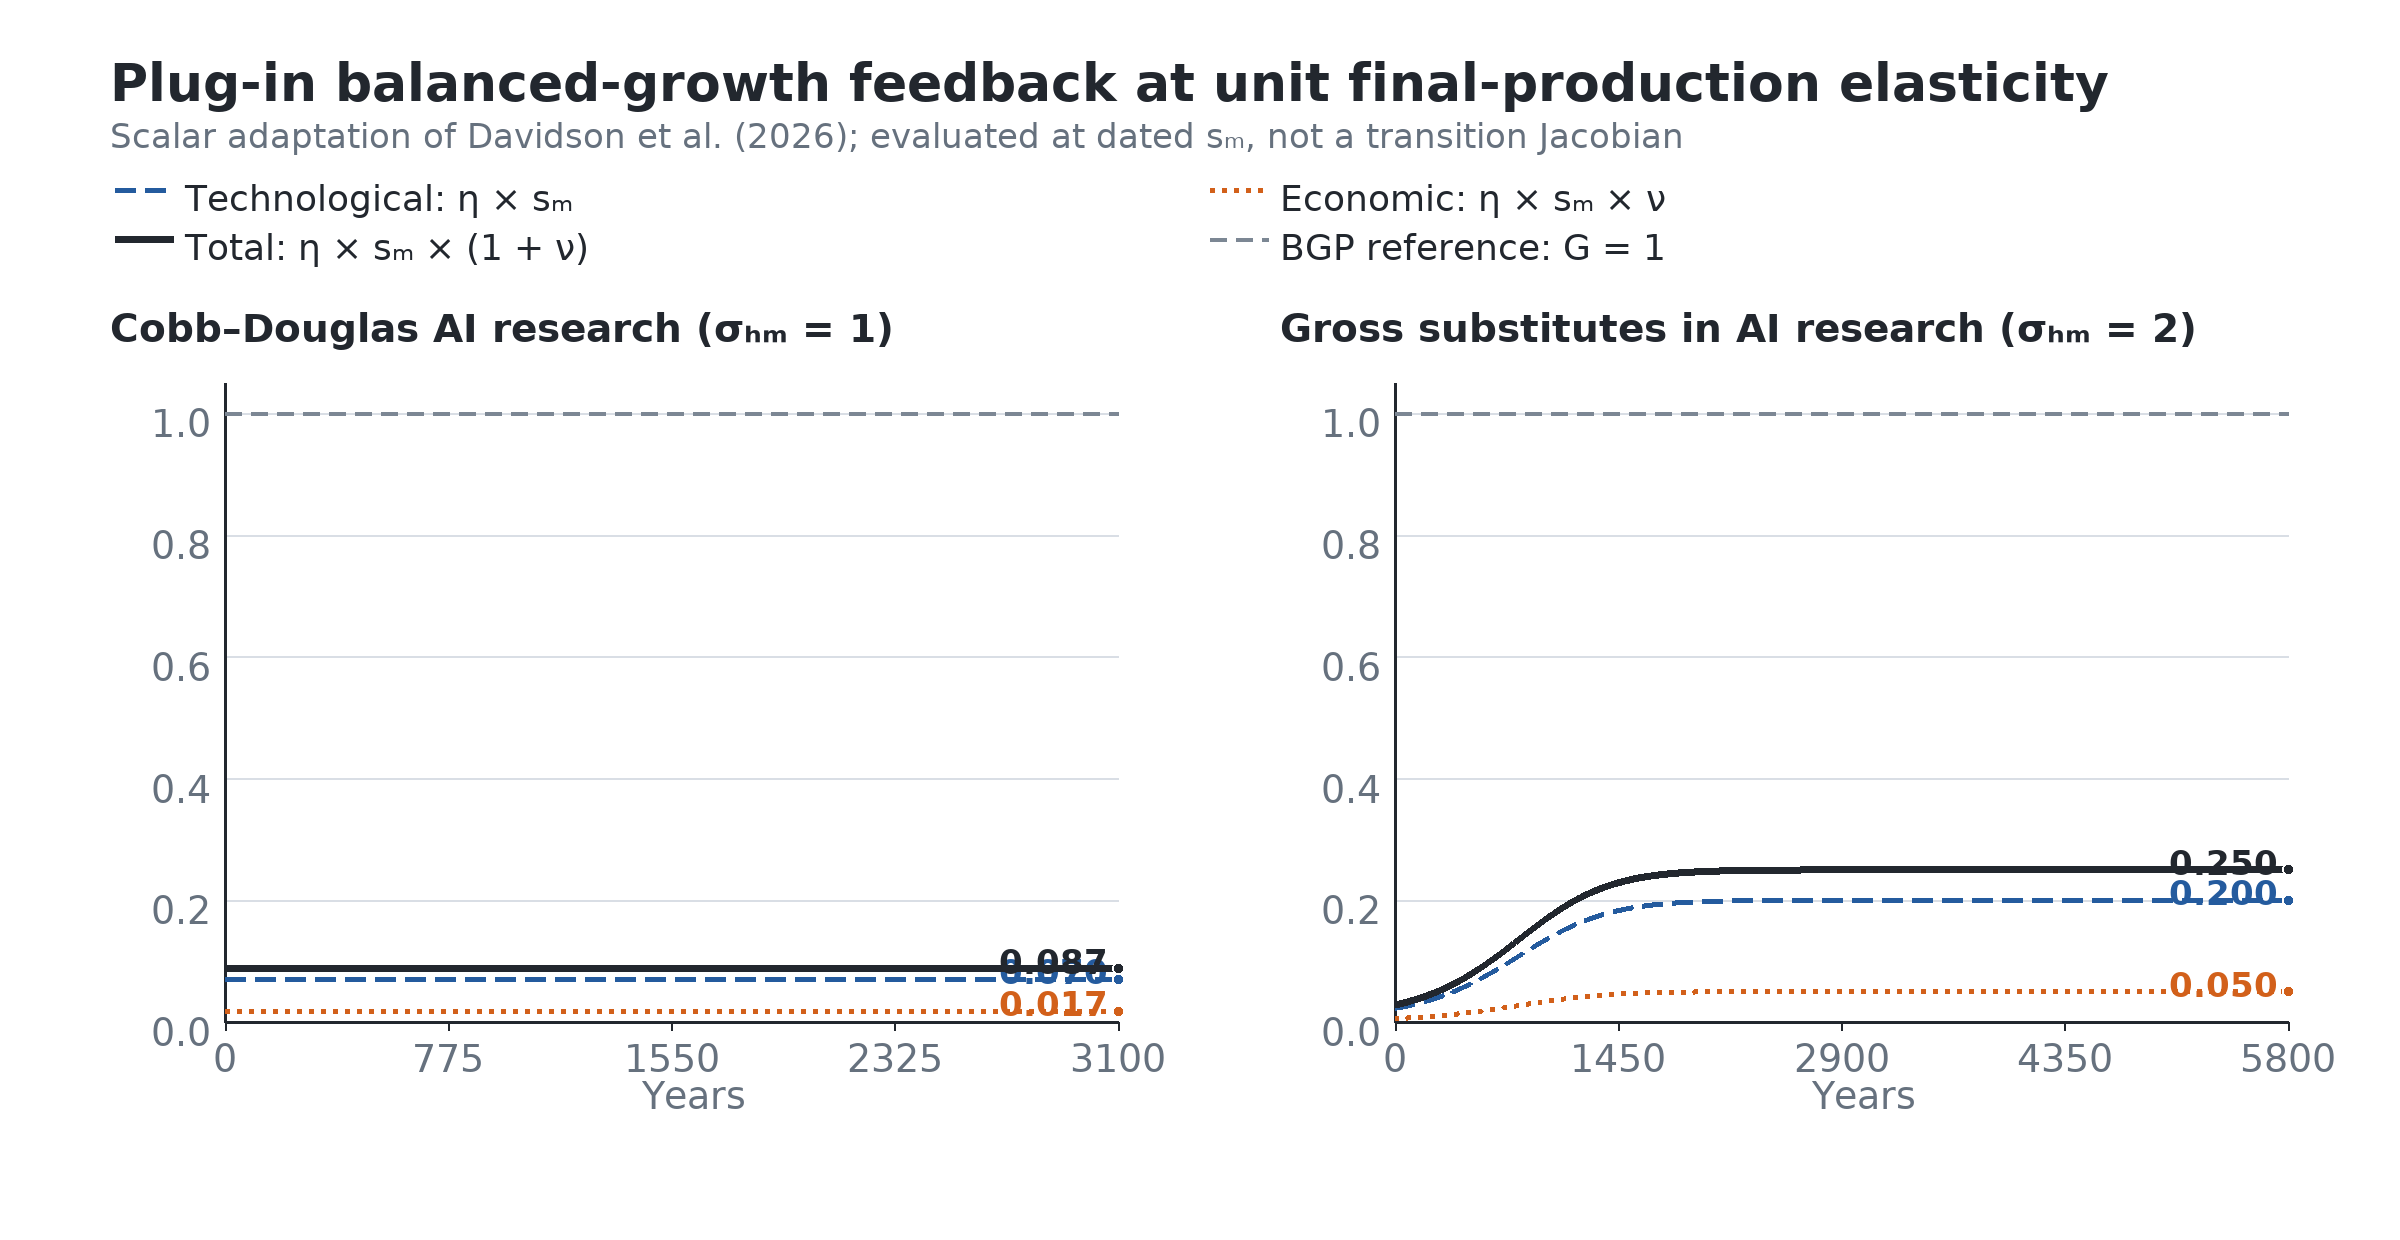
\includegraphics[width=\textwidth]{figures_axm/axm_unit_elasticity_feedback_diagnostic.png}
\caption{Plug-in balanced-growth feedback accounting evaluated at \(s_M(t)\)
along the two unit-elasticity finite-horizon candidate paths. The construction is
a scalar adaptation of \citet{davidsonetal2026}, not the dated feedback Jacobian.
The horizontal line at one is the critical value for the balanced-growth
accounting in equation~\eqref{eq:axm-feedback-matrix}, not a sufficient condition
for explosive equilibrium dynamics.}
\label{fig:axm-feedback-diagnostic}
\end{figure}

\subsection{Acceptance tests, independent audits, and limits of the evidence}

For every reported unit-elasticity path and every horizon-robustness path, the
canonical code recomputes the dated static allocation and records the technology,
goods-market, labor-market, monopoly, research, and dynamic residuals. It also
checks the monopoly second-order condition and stores all six horizon paths,
rather than retaining only their initial jumps. The row-by-row audit reconstructs
\(X=AU\), the service \(AM\), the CES research-input index, the capability law,
both research first-order conditions, and the costate term
\(-\eta s_M\dot A/A\). The collocation derivative, rather than a plotted finite
difference, is used for the unit-elasticity dynamic residuals.

Table \ref{tab:axm-residuals} reports the solver-side diagnostics for the two
baseline unit-elasticity paths. Static identities and first-order conditions have
errors below \(10^{-10}\) in the stored solver diagnostics. The larger entries are
collocation residuals in the differential equations and remain close to
\(10^{-5}\).

\begin{table}[H]
\centering
\small
\caption{Unit-elasticity path diagnostics}
\label{tab:axm-residuals}
\begin{tabular}{lcc}
\toprule
Diagnostic & \(\sigma_{HM}=1\) & \(\sigma_{HM}=2\)\\
\midrule
Maximum goods-market residual & \(2.2\times10^{-16}\) & \(3.3\times10^{-16}\)\\
Maximum labor-market residual & \(3.6\times10^{-15}\) & \(7.1\times10^{-15}\)\\
Maximum technology log error & \(1.4\times10^{-14}\) & \(2.4\times10^{-12}\)\\
Maximum factor-price error & \(1.8\times10^{-15}\) & \(7.1\times10^{-15}\)\\
Maximum research-duality error & \(1.8\times10^{-14}\) & \(4.9\times10^{-11}\)\\
Maximum monopoly-FOC log error & \(1.6\times10^{-14}\) & \(2.7\times10^{-14}\)\\
Maximum research-FOC log error & \(1.8\times10^{-14}\) & \(2.4\times10^{-11}\)\\
Maximum dynamic path residual & \(1.2\times10^{-6}\) & \(5.4\times10^{-6}\)\\
Maximum horizon-induced initial-jump range & \(2.6\times10^{-9}\) & \(7.4\times10^{-9}\)\\
Minimum monopoly second-order margin & 0.1160 & 0.1160\\
Absolute terminal capability-growth error & \(6.1\times10^{-7}\) & \(4.1\times10^{-9}\)\\
Absolute terminal per-capita-output-growth error & \(5.4\times10^{-8}\) & \(8.2\times10^{-10}\)\\
Terminal automated research-expenditure share & 0.3500 & 1.00000\\
Log household terminal-TVC proxy & -85.23 & -160.83\\
Log developer terminal-TVC proxy & -87.54 & -163.14\\
\bottomrule
\end{tabular}
\end{table}

The horizon-induced range is the larger of the ranges of \(\log C(0)\) and
\(\log q(0)\), measured in log points. The terminal growth errors are absolute
differences between annual rates expressed as decimals. Across all six horizon
paths, the largest reconstructed static-equation error is
\(4.9\times10^{-11}\). The largest differential-equation residual is
\(6.6\times10^{-6}\), and both imposed terminal-ratio errors are below
\(8.0\times10^{-8}\). Every saved quantity remains positive, and the monopoly
second-order margin is strictly positive.

The two TVC entries evaluate the expressions in equation~\eqref{eq:axm-tvc} at
the finite terminal date. Their finite magnitudes depend on normalization; only
convergence to zero is invariant. They are truncation diagnostics, not direct
verification of a limit as \(t\to\infty\). Under the analytical balanced-growth
continuation, if it exists, both objects decay at rate \(\rho-n>0\).

The complementary-input calculations have a separate auditor, which does not
import the solver. Its source is
\path{scripts/audit_axm_complements.py}. It
reconstructs the static equations from the saved rows and estimates the four log
derivatives with centered local polynomials. Acceptance requires small static and
dynamic residuals, positive and interior allocations, a positive monopoly
second-order margin, no active saved clipping or fallback, accurate imposed
terminal restrictions, convergence of non-imposed terminal quantities, and
stable initial jumps across horizons.
Across the two displayed \(T=4{,}500\) paths, the largest reconstructed static
error is \(5.32\times10^{-11}\), the largest independently differentiated
dynamic error is \(5.20\times10^{-7}\), and the largest monopoly first-order
condition error is \(3.14\times10^{-10}\). Across all six cold starts, the
largest solver root-mean-square residual is \(9.36\times10^{-7}\), the largest
independently differentiated dynamic error is \(8.35\times10^{-7}\), and the
largest horizon-induced initial-jump range is \(2.92\times10^{-7}\) log points.
Every prespecified acceptance gate
passes, including the finite-date transversality proxies. These proxies remain
truncation diagnostics and do not establish the infinite-horizon limits.

The high-substitution calculation is checked by
\path{scripts/audit_axm_high_sigma.py}. This auditor reconstructs all
technologies, prices, first-order conditions, income shares, the household
budget, market clearing, and the four dynamic right-hand sides without calling
the solver's static-equilibrium routine. It also differentiates the four
log-state paths independently on a compact calendar window. Acceptance requires positivity,
a strictly positive monopoly second-order margin, no active saved clipping,
small equation residuals, stable initial jumps, convergence on common calendar
and event-time windows, stability of the imposed terminal ratios, convergence of
the non-imposed terminal quantities, and stabilization of
\eqref{eq:axm-singularity-tail-estimate}. All prespecified gates pass for
\(z_T=16,32,64,128\).

\begin{sloppypar}
The simulation files and residual summaries are stored in
\path{numerical_axm}. The canonical fixed-horizon solver is
\path{scripts/simulate_axm_equilibrium.py}; the complementary-input runner and
the free-boundary solver are
\path{scripts/simulate_axm_complements_equilibrium.py} and
\path{scripts/simulate_axm_high_sigma_equilibrium.py}. The mapping from manuscript
equations to solver objects and diagnostics is stored in
\path{numerical_axm/equilibrium_equation_map.csv}. Scripts without the
\texttt{axm} designation that solve or simulate an equilibrium implement the
earlier research specification and do not generate evidence used in this paper.
Plotting scripts read accepted paths and do not solve an additional equilibrium
system. In particular,
\path{scripts/plot_axm_distribution_decomposition.py} verifies the hashes in
all three accepted audit manifests, reconstructs the six components of
\eqref{eq:axm-consolidated-distribution} from dated prices and quantities, and
checks nonnegativity and accounting closure before drawing the cross-regime
figure.
The reported reruns used Python 3.12.13, NumPy 2.5.2, SciPy 1.18.0, and Pillow
12.3.0. These versions are pinned in \path{requirements-numerical.txt}.
Floating-point arithmetic and platform-specific rendering can still prevent
bit-for-bit identity across computing environments; acceptance is based on the
reported numerical tolerances and equation audits rather than file identity
alone.
Within \path{numerical_axm}, diagnostic values and pass/fail status are stored in
\path{audit_report.csv}, \path{complements_acceptance_report.csv}, and
\path{high_sigma_sigma150_validated_acceptance_report.csv}. The last two reports
also state their numerical thresholds, and their manifests record the audited
inputs. Unit-elasticity thresholds are defined in
\path{scripts/audit_axm_model.py};
\path{unit_elasticity_audit_manifest.json} binds its four numerical inputs to
the current audit and generator scripts by SHA-256 hash.
\end{sloppypar}

Convergence of the collocation routine establishes only that a finite-horizon or
finite-boundary discretization satisfies its equations and imposed boundary
conditions within the reported tolerances. Agreement of an imposed terminal
ratio is not independent validation. The overidentifying evidence comes from the
dated residuals, non-imposed quantities, and stability across horizons or
boundaries. Finite terminal values of the two transversality expressions are
recorded, but they do not prove their infinite-horizon limits. The
unit-elasticity sufficiency result applies only to an admissible exact continuation
satisfying the full system and both transversality conditions. The
complementary-input calculations are finite-horizon approximations to candidate
paths. The
gross-substitutes calculations are finite-boundary approximations to a
conditional pre-singular branch of the necessary conditions; they do not establish
an infinite-horizon equilibrium, global stability, uniqueness, or reachability
from arbitrary initial states.

Table \ref{tab:axm-high-sigma-convergence} and Figure
\ref{fig:axm-high-sigma-ratios} report the free-boundary diagnostics removed from
the sequence of economic outcomes in the main text. Only \(C/Y\), \(qA/K\), and
terminal \(Y/K\) are imposed at each boundary. The other terminal quantities and
the agreement of overlapping path segments are overidentifying checks on the
conditional asymptotic characterization.

\begin{table}[H]
\centering
\small
\caption{Free-boundary convergence and terminal ratios,
\(\sigma_{XL}=1.5,\ \sigma_{HM}=2\)}
\label{tab:axm-high-sigma-convergence}
\begin{tabular}{lccccc}
\toprule
Terminal \(Y/K\) & 16 & 32 & 64 & 128 & Limit\\
\midrule
Estimated \(T^*\) & 1669.005 & 1669.021 & 1669.025 & 1669.026 & ---\\
\(g_A/(Y/K)\) & 0.02265 & 0.02296 & 0.02313 & 0.02322 & 0.02332\\
\(U/Y\) & 0.44889 & 0.44890 & 0.44890 & 0.44890 & 0.44890\\
\(M/Y\) & 0.03081 & 0.03123 & 0.03146 & 0.03159 & 0.03172\\
\((\dot K+\delta K)/Y\) & 0.28357 & 0.28315 & 0.28291 & 0.28279 & 0.28266\\
\(s_X\) & 0.999986 & 0.999998 & 1.000000 & 1.000000 & 1\\
\(wN/Y\) & \(9.37\times10^{-6}\) & \(1.65\times10^{-6}\) & \(2.91\times10^{-7}\) & \(5.16\times10^{-8}\) & 0\\
\bottomrule
\end{tabular}

\medskip
\parbox{0.94\textwidth}{\footnotesize \emph{Notes:} The estimated \(T^*\) is
measured in model time. All remaining entries are ratios expressed as fractions,
so, for example, 0.02265 corresponds to 2.265 percent. The final column reports
the conditional analytical limit.}
\end{table}

\begin{figure}[H]
\centering
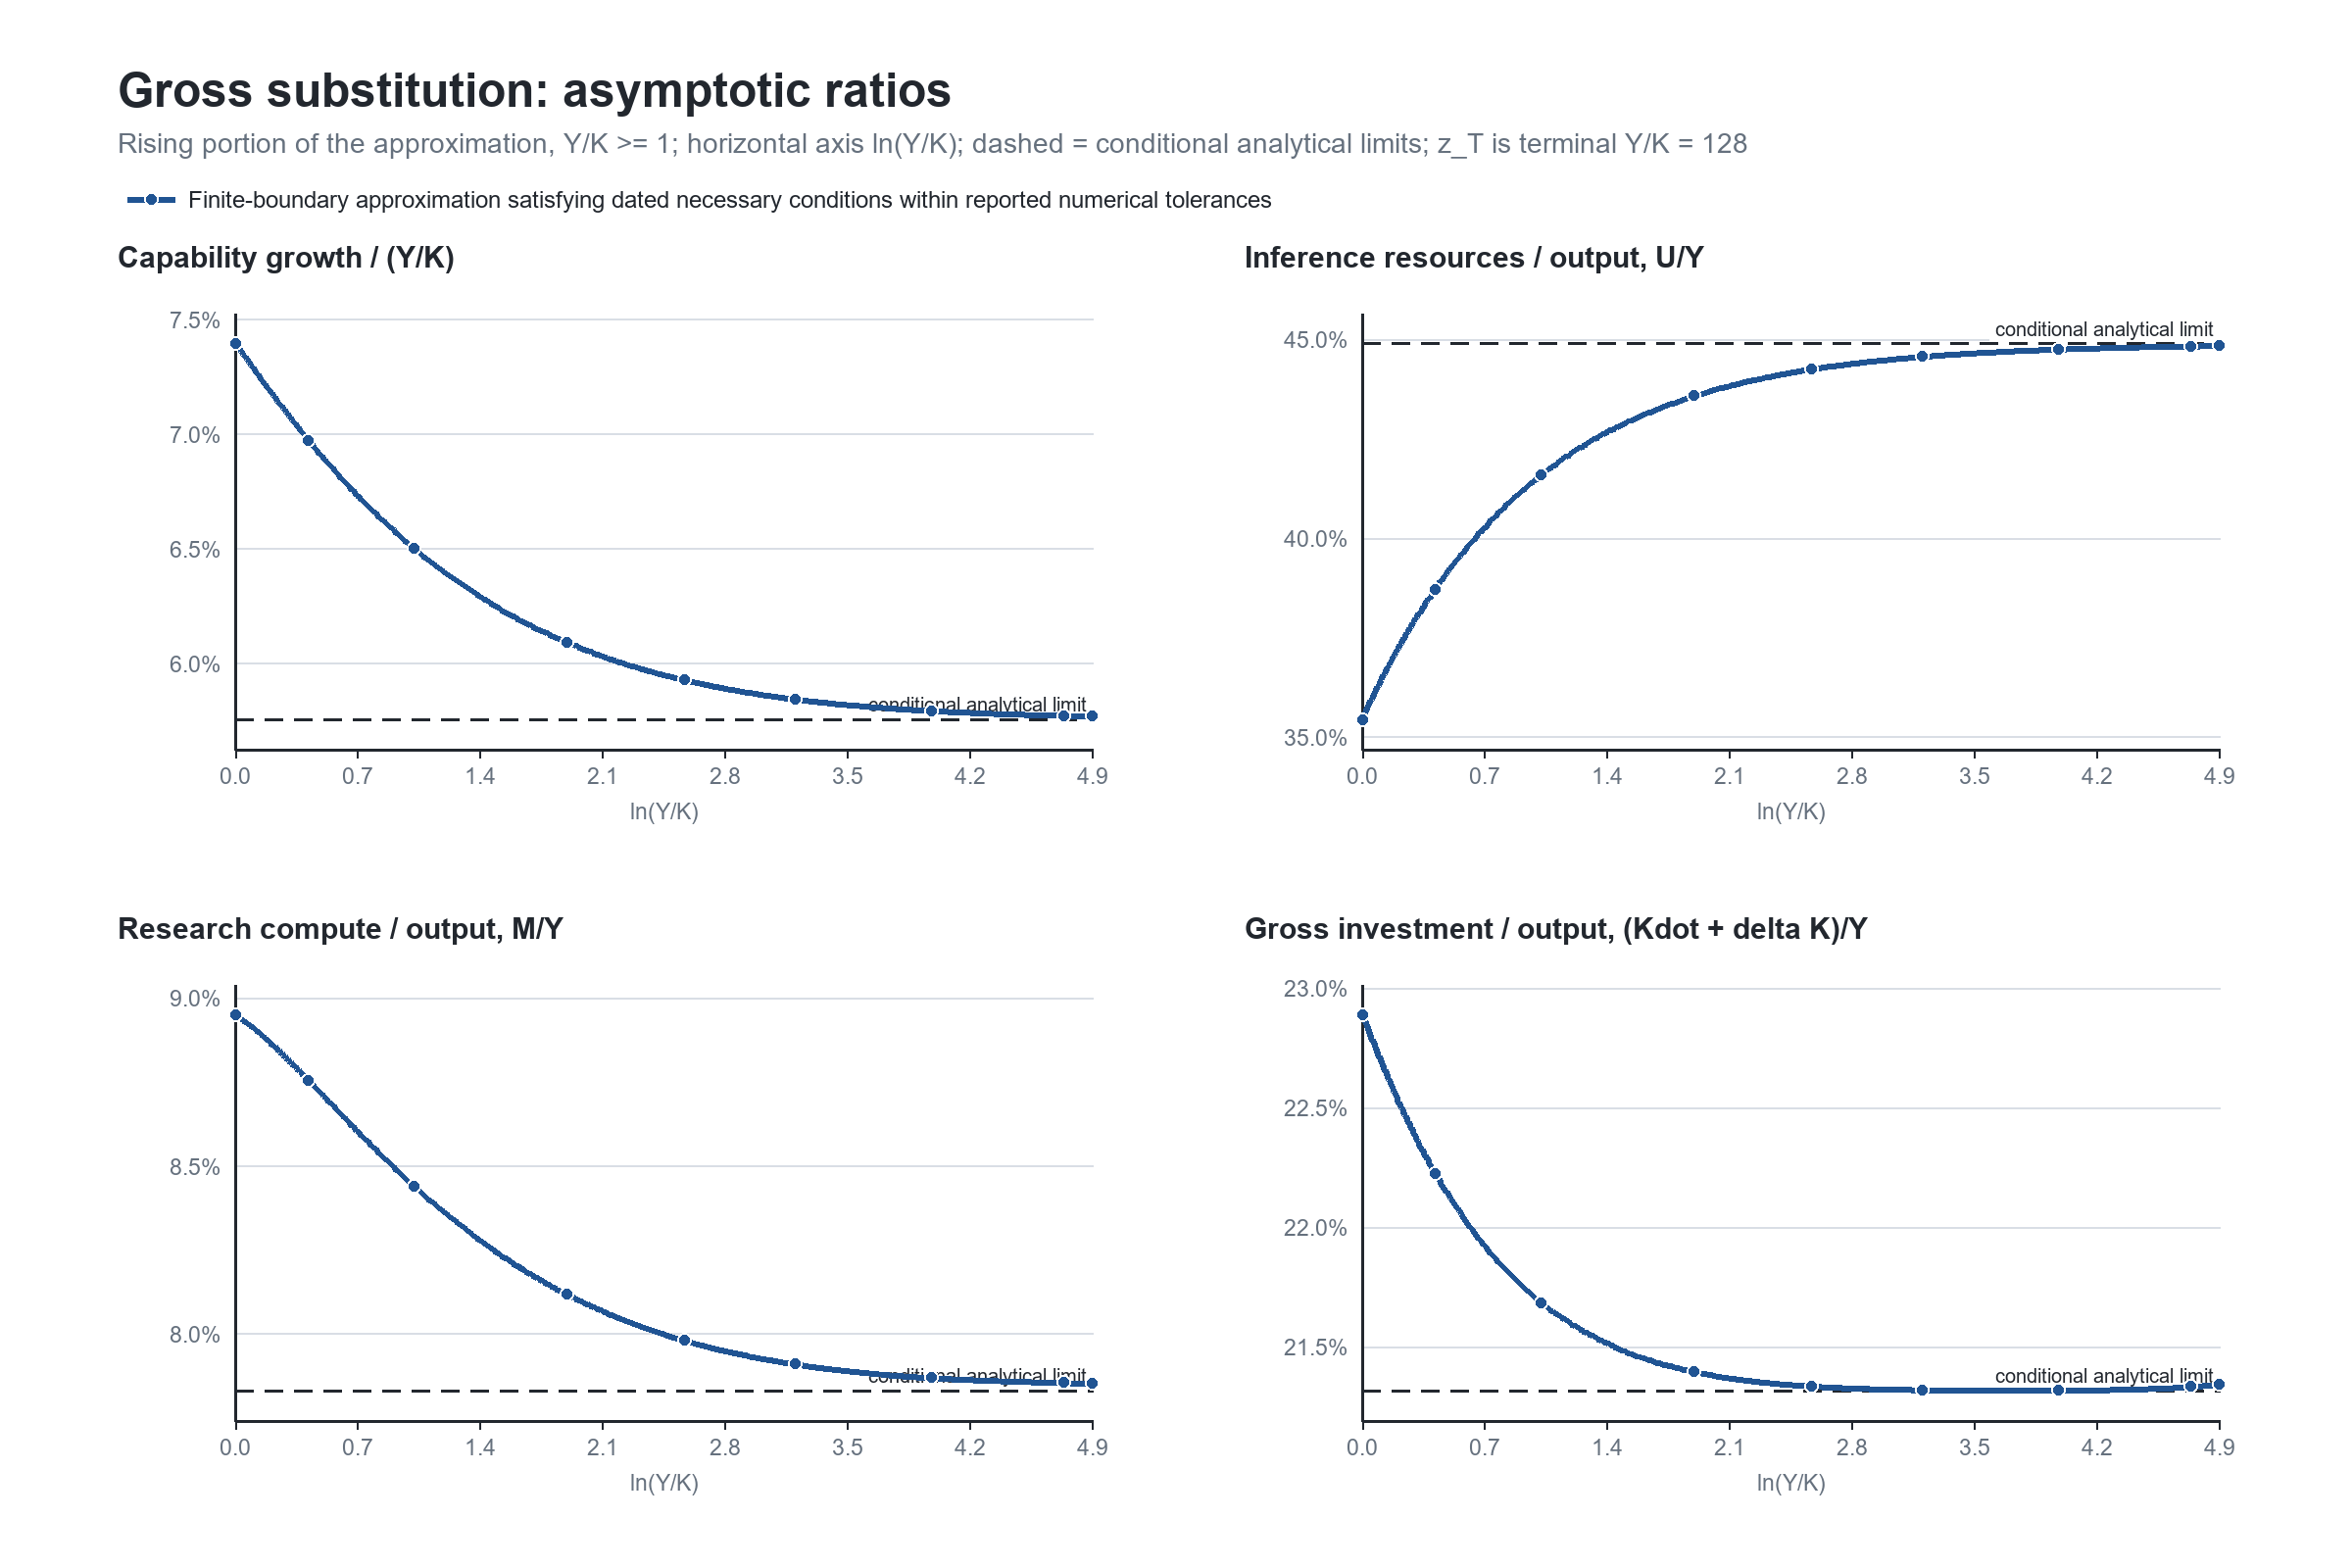
\includegraphics[width=\textwidth]{figures_axm/high_sigma_validated_asymptotic_ratios.png}
\caption{Selected non-imposed ratios along the rising branch of \(Y/K\). The
horizontal axis is \(\ln(Y/K)\); dashed lines are the conditional analytical
limits in Conditional Result \ref{prop:axm-singular-limit}. Vertical axes use
linear percentages with panel-specific ranges.}
\label{fig:axm-high-sigma-ratios}
\end{figure}

\begin{figure}[H]
\centering
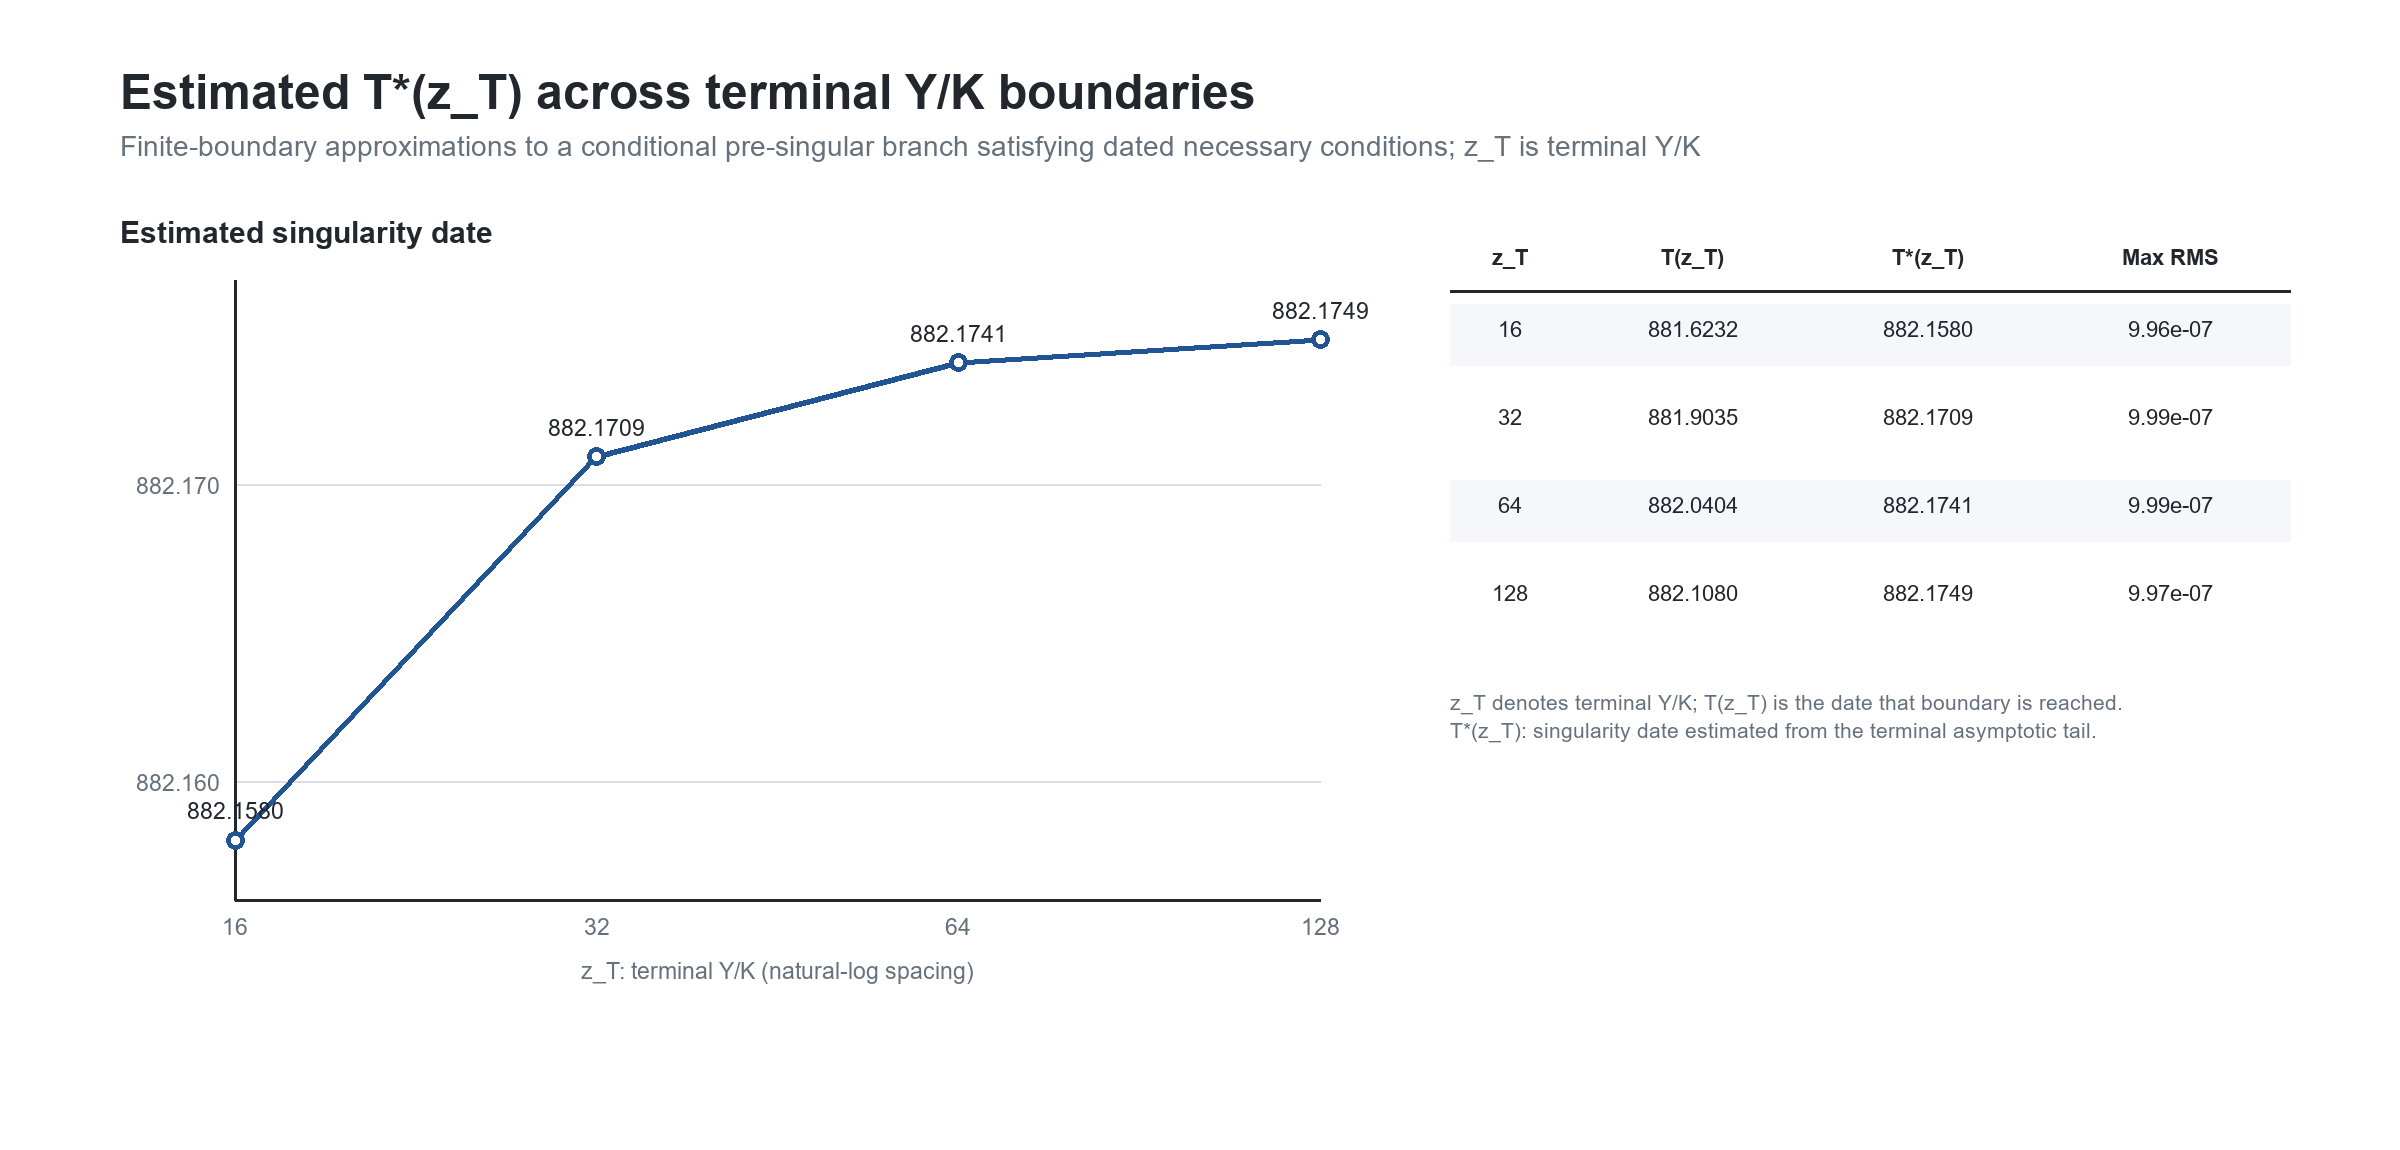
\includegraphics[width=\textwidth]{figures_axm/high_sigma_validated_boundary_convergence.png}
\caption{Free-boundary convergence diagnostic, where
\(z_T\equiv(Y/K)(T)\). \(T(z_T)\) is the date at which the approximation reaches
its artificial terminal boundary. The graphic writes \(T^*(z_T)\) for the tail
estimate \(\widehat T(z_T)\) in
\eqref{eq:axm-singularity-tail-estimate}. The residual column reports the maximum
collocation root-mean-square error.}
\label{fig:axm-high-sigma-boundary-convergence}
\end{figure}
